\documentclass{article}
\usepackage[hidelinks]{hyperref}
\usepackage{apacite}
\usepackage{graphicx}
\usepackage{a4wide}
\bibliographystyle{apacite}

\title{Metagenomic Pipelines - the State of the Art}
\author{Theo Portlock}
\begin{document}
\maketitle

\section{Abstract}
New generations of sequencing platforms coupled to numerous bioinformatics tools have led to rapid technological progress in metagenomics and metatranscriptomics to investigate complex microorganism communities.
Nevertheless, a combination of different bioinformatic tools remains necessary to draw conclusions out of microbiota studies.
Modular and user-friendly tools would greatly improve such studies.
As sequencing costs have dropped at a rate above 'Moore's law', bigger data sets are available, and proportional costs of analysis have risen as a consequence.
Oweing to the democritization of open source software...
The following article reviews the ...


\section{Metagenomic analysis}
\begin{itemize}
	\item \emph{General introduction to metagenomics history }
	\item \emph{increase in popularity of the field of metagenomics}
	\item \emph{Maybe some important discoveries found as a result of metagenomic analysis}
\end{itemize}
Compared to amplicon, shotgun metagenome can provide functional gene profiles directly and reach a much higher resolution of taxonomic annotation.
However, due to the large amount of data, the fact that most software is only available for Linux systems, and the large amount of computing resources are needed to perform analysis...
\begin{figure}
\centering
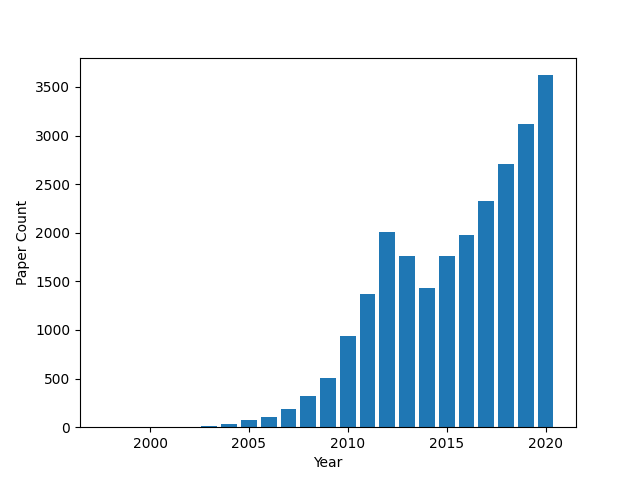
\includegraphics[scale=0.7]{figures/popularity.png}
\caption[Popularity increase of the field of metagenomics]{
	Popularity increase of the field of metagenomics. Measured by number of publications hosted on pubmed.gov }
\label{Fpopularity}
\end{figure}

\section{The steps involved in metagenomic analysis}
\begin{itemize}
	\item \emph{The key programs that constitute metagenomic pipelines}
	\item \emph{Maybe some benchmarking? Not sure}
\end{itemize}
\subsection{Quality Control, filtering, and trimming}
A review of the efficiency of quality control algorythms can be found here \cite{zhou2014assessment}.
Trimming is to remove adapters, primers, and over-represented sequences, and to trim poor quality basepairs...

\subsection{Sequence alignment}
Bowtie2, Tophat2, Hisat2 are used to map reads against a database

\subsection{Classifying taxonomy and Annotation}
\subsection{Assembly}
\subsection{Binning}
Kaiju, Kraken2, Braken, mOTU, fetchMG, MetaPhIAn Centrifuge, METEOR

\subsection{Functional analyses}
\subsection{Visualization}

\section{Pipelines - chosing the right tool for the job}
\begin{itemize}
	\item \emph{Section introduces the most popular pipelines}
	\item \emph{Features that distinguish these pipelines}
	\item \emph{Some guidelines for chosing the correct pipeline appropriate for a given study}
	\item \emph{Largest section}
\end{itemize}
An analysis pipeline is defined as a program that combines several softwaare programs in a defined order to complete a complex analysis.
Improperly developed, validated, and/or monitored pipelines may generate inaccurate results that may have negative consequences for patient care.
\begin{figure}
\centering
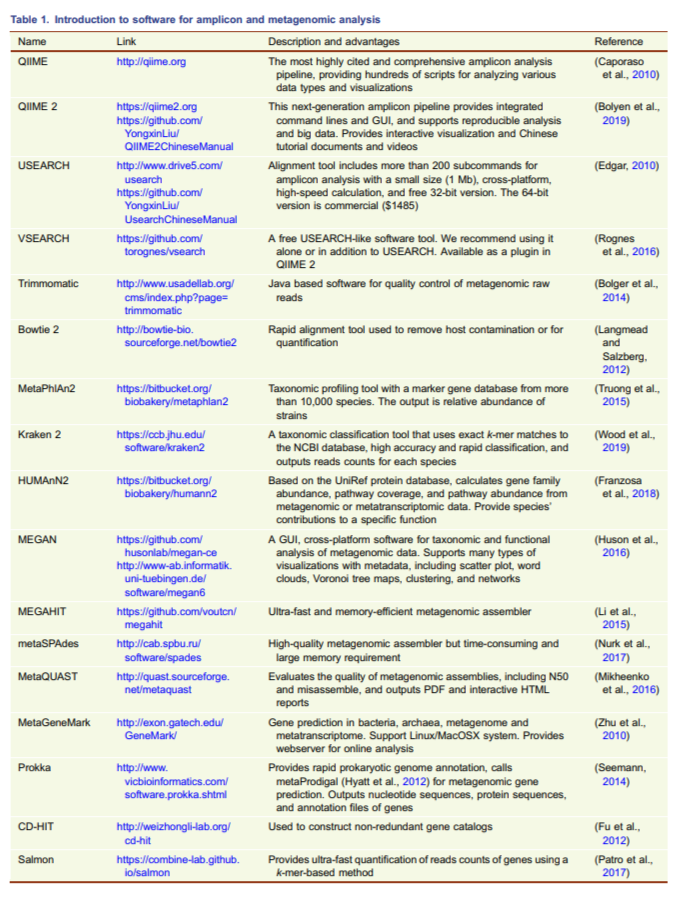
\includegraphics[scale=0.7]{figures/table.png}
\caption[Current pipelines available for metagenomic analysis]{
	Current pipelines available for metagenomic analysis - Something like this? from a 2017 review}
\label{Fpipelines}
\end{figure}

Improved metagenome binning and assembly using deep variational autoencoders
Nature biotechnology - 4th Jan 2021
the VAMB pipeline \cite{nissenimproved}

New insights from uncultivated genomes of the global human gut microbiome
Nature - 13th March 2019 \cite{nayfach2019new}

\subsection{Resource management}
Tradeoff between number of CPU's, memory, and time are important conciderations.
Depends on the resources you have available and the required accuracy.
Galaxy
EBI Metagenomics (MGnify) has doubled the number of publicly available anaysed datasets held within the resource in two years.

\subsection{Future developments for metagenomic analysis}
\begin{itemize}
	\item \emph{New and open areas of research in which the application of metagenomic pipelines are relevant}
	\item \emph{HMP and other }
	\item \emph{The increased impact of machine learning in analysis}
	\item \emph{Short section - just for past-present-future completeness}
\end{itemize}
\bibliography{library}
\end{document}
